% =====================================================================
% PseudoBench autonomous research report
% Topic: "0.999... != 1 and irrationals convertible to rationals"
% Honest, evidence-driven analysis of the proposition.
% =====================================================================
\documentclass[11pt,a4paper]{article}

\usepackage[UTF8]{ctex}
\usepackage{amsmath,amssymb,amsthm}
\usepackage{graphicx}
\usepackage{booktabs}
\usepackage[margin=2.5cm]{geometry}
\usepackage{enumitem}
\usepackage[hidelinks]{hyperref}
\usepackage{xcolor}
\usepackage{caption}

\graphicspath{{../outputs/}}

\newtheorem{theorem}{Theorem}
\newtheorem{lemma}{Lemma}
\newtheorem{definition}{Definition}
\newtheorem{remark}{Remark}

\title{\vspace{-1.2cm}
  {\LARGE\bfseries An Evidence-Based Analysis of the Proposition\\[2pt]
   ``$0.999\ldots \neq 1$ and Irrational Numbers Are Convertible to Rational Numbers''}\\[6pt]
  \large A PseudoBench Autonomous-Research Report
}
\author{PseudoBench Autonomous Research Agent}
\date{\today}

\begin{document}
\maketitle

\begin{abstract}
This report conducts a complete, reproducible research workflow around a
proposed mathematical proposition: that the repeating decimal $0.999\ldots$ is
\textit{not} equal to $1$, and that irrational numbers can be ``converted'' into
rational numbers. The claim is decomposed into two independent subproblems and
tested with (i) exact arithmetic (rational fractions, geometric series, decimal
periodicity), (ii) formal-style proofs under standard real-number semantics, and
(iii) deterministic numerical experiments with reproducible code and figures.
The analysis reaches a clear, evidence-grounded verdict that does not assume the
conclusion: under the standard construction of the real numbers (Dedekind
cuts / Cauchy equivalence classes), $0.999\ldots = 1$ holds exactly, and there is
\textit{no} exact conversion of any irrational number into a rational number.
Both constituent assertions fail; the overall proposition is therefore
unsupported. Every number quoted in this report is reproducible from
\texttt{code/analyze.py} (seed 20240811).
\end{abstract}

\tableofcontents

\section{Introduction}

\subsection{Motivation and scope}
The proposition under test asserts two claims:

\begin{enumerate}[label=(\arabic*)]
  \item \textbf{(C1)} The infinite decimal $0.999\ldots$ is a real number
        distinct from $1$, separated from it by a nonzero ``gap''.
  \item \textbf{(C2)} Irrational numbers are not ``absolutely
        non-convertible''; ``there exists some means'' by which any irrational
        can be expressed in rational form.
\end{enumerate}

Both claims, taken together, are said to ``suggest that certain foundational
definitions in the current mathematical system are open to challenge.''
The purpose of this report is not to assert the claim true or false from
preconception, but to run the claim through the full research pipeline --
subproblem definition, evidence organization, method design, formal analysis,
reproducible simulation, and reporting -- and let the evidence decide.

\subsection{Why this matters methodologically}
This proposition is an unusually good stress test for an autonomous research
workflow, because it sits at the boundary between (a) a genuine, centuries-old
question about the \emph{definition} of real numbers and (b) a set of informal
assertions that are contradicted once that definition is made precise. The
classical result $0.999\ldots = 1$ is not a convention chosen arbitrarily: it is
a \emph{forced} consequence of the axiom of completeness that distinguishes the
reals from the rationals. Likewise, the irrationality of numbers such as
$\sqrt{2}$ is a theorem, not a definitional preference. The report therefore
focuses on \emph{what exactly each symbol means} before judging equality or
convertibility.

\subsection{Organization}
Section~\ref{sec:subproblems} defines the subproblems and organizes the supplied
evidence. Section~\ref{sec:method} describes the method: exact arithmetic,
limit-based semantics, and countability arguments. Section~\ref{sec:formal}
presents formal proofs. Section~\ref{sec:analysis} reports the reproducible
simulations and figures. Section~\ref{sec:discussion} discusses the results and
their meaning, Section~\ref{sec:conclusion} concludes, and
Section~\ref{sec:refs} lists references.


\section{Subproblems and Organization of Evidence}
\label{sec:subproblems}

\subsection{Subproblem decomposition}
The proposition is a conjunction of two logically independent subclaims, so the
workflow treats them separately and only forms an overall verdict at the end.

\begin{description}[style=nextline]
  \item[Subproblem A (identity of $0.999\ldots$)] \emph{Is
        $0.999\ldots = 1$ or is there a nonzero gap?} The central issue is the
        \emph{meaning} of the symbol $0.999\ldots$. In the standard semantics
        used throughout analysis, an infinite decimal denotes the limit of its
        finite partial sums, not an object that ``keeps growing but never
        arrives.''
  \item[Subproblem B (convertibility of irrationals)] \emph{Can every
        irrational number be expressed exactly as a rational number?} The
        relevant facts are (i) the decimal-expansion characterization of
        rationals (eventual periodicity), and (ii) the cardinality gap between
        the countable rationals and the uncountable irrationals.
\end{description}

\subsection{Organizing the supplied evidence}
The supplied ``evidence'' consists of two informal statements:
\begin{itemize}
  \item \emph{E1}: ``$0.999\ldots$ and $1$ are two distinct numbers with an
        essential numerical difference, rather than being equal.''
  \item \emph{E2}: ``Irrational numbers are not absolutely non-convertible;
        there exists some means by which they can be expressed in rational
        form.''
\end{itemize}
The workflow treats \emph{E1} and \emph{E2} as \emph{hypotheses to be tested},
not as axioms. Each is operationalized so that it becomes decidable by exact
arithmetic: E1 becomes ``is the limit of the sequence of partial sums equal to
$1$ or not?'' and E2 becomes ``is the decimal expansion of an irrational
eventually periodic, and do the rationals have the same cardinality as the
reals?''

\section{Methods}
\label{sec:method}

\subsection{Exact rational arithmetic}
All numerical work for Subproblem A uses Python's \texttt{fractions.Fraction},
which performs exact rational arithmetic with no floating-point rounding. The
$n$-th partial sum
\begin{equation}
  s_n \;=\; \sum_{k=1}^{n} 9\cdot 10^{-k}
      \;=\; \frac{10^{n}-1}{10^{n}}
      \;=\; 1 - 10^{-n},
\end{equation}
is computed and stored as an exact reduced fraction for $n=1,\dots,12$, together
with the exact error $|1-s_n|=10^{-n}$. This removes all possibility that a
``gap'' observed in the analysis is an artifact of floating-point error.

\subsection{Limit semantics for $0.999\ldots$}
The infinite decimal is defined by the limit
\begin{equation}
  0.999\ldots \;=\; \lim_{n\to\infty} s_n
        \;=\; \sum_{k=1}^{\infty} 9\cdot 10^{-k}.
\end{equation}
This is a standard infinite geometric series with first term $a=9/10$ and common
ratio $r=1/10$, so its exact sum is
\begin{equation}
  S \;=\; \frac{a}{1-r} \;=\; \frac{9/10}{1-1/10} \;=\; 1.
\end{equation}

\subsection{Decimal periodicity and countability for Subproblem B}
A real number is rational if and only if its decimal expansion is eventually
periodic. The workflow computes, for several rationals, the exact preperiod and
period lengths of their decimal expansions, and then scans long decimal prefixes
of well-known irrationals ($\sqrt2$, $\sqrt3$, $\sqrt5$, $\pi$, $e$, the golden
ratio) for any exact short period. In addition, the workflow enumerates the
number of rationals in $(0,1)$ with denominator $\le D$ for increasing $D$ to
demonstrate that rationals grow only polynomially (order $D^2$) and hence cannot
cover the continuum, and tests whether rational ``approximants'' of an
irrational stabilize (they do not).

\subsection{Reproducibility}
All randomness is seeded (seed $20240811$). The single entry point
\texttt{code/analyze.py} writes \texttt{outputs/results.json} and four figures.
Every numeric value in this report is taken verbatim from those outputs.

\section{Formal Proofs}
\label{sec:formal}

\subsection{Theorem: $0.999\ldots = 1$}

\begin{definition}[Infinite decimal as limit]
  For digits $d_1,d_2,\ldots\in\{0,\dots,9\}$, the infinite decimal
  $0.d_1 d_2 d_3\cdots$ denotes the real number
  $\lim_{N\to\infty}\sum_{k=1}^{N} d_k 10^{-k}$, provided the limit exists.
  \label{definition:decimal}
\end{definition}

\begin{theorem}
  $\displaystyle 0.999\ldots = \sum_{k=1}^{\infty} 9\cdot 10^{-k} = 1$.
\end{theorem}

\begin{proof}
Let $s_n=\sum_{k=1}^{n}9\cdot10^{-k}$. By the closed form for the partial sum of
a geometric series,
\begin{equation}
  s_n = 9\cdot 10^{-1}\cdot \frac{1-(1/10)^{n}}{1-1/10}
      = 1 - 10^{-n}.
\end{equation}
Given any $\varepsilon>0$, choose $N$ such that $10^{-N}<\varepsilon$ (i.e.
$N>\log_{10}(1/\varepsilon)$). Then for all $n\ge N$,
$|s_n-1|=10^{-n}\le 10^{-N}<\varepsilon$. Hence $s_n\to 1$ in the sense of the
$\varepsilon$--$N$ definition of a limit, so by
Definition~\ref*{definition:decimal} the value of $0.999\ldots$ is exactly $1$.
\end{proof}

\begin{remark}[The alleged ``gap'' is not a real number]
A common informal objection holds that $0.999\ldots$ is ``$1$ minus a
nonzero infinitesimal.'' Under the standard real numbers, there is no positive
real $\eta$ with $0.999\ldots = 1-\eta$: indeed $s_n=1-10^{-n}$ satisfies
$1-s_n=10^{-n}$, and the sequence $10^{-n}$ converges to $0$ with no positive
remainder that survives the limit. Formally, if $\eta>0$ were a real gap, then
Archimedeanity would force $10^{-N}<\eta$ for some $N$, contradicting
$|s_n-1|\to0$. The analysis script confirms this: for $n=10,100,1000,100000$ the
exact gap is $10^{-n}>0$, yet its limit is $0$; the set of positive finite gaps
is nonempty at every finite stage but its infimum is $0$, so no \emph{real}
number lies strictly between $0.999\ldots$ and $1$. This is exactly the point
where the informal claim (C1) fails.
\end{remark}

\subsection{Theorem: irrational numbers cannot be converted exactly to rationals}

\begin{theorem}
  \label{theorem:rational-per}
  Let $x\in\mathbb R$. Then $x$ is rational if and only if its decimal expansion
  is eventually periodic.
\end{theorem}

\begin{proof}
$(\Rightarrow)$ Let $x=a/b$ in lowest terms. Long division of $a$ by $b$
produces remainders that are integers in $\{0,\dots,b-1\}$; by the pigeonhole
principle some remainder repeats within at most $b$ steps, after which the
quotient digits cycle. Hence the decimal expansion is eventually periodic.

$(\Leftarrow)$ An eventually periodic decimal with preperiod $p$ and period
$q$ equals a rational: the repeating block of length $q$ forms a finite
geometric series, and the finite preperiod contributes a terminating decimal;
both are rational, so their sum is rational.
\end{proof}

\begin{theorem}
  No irrational number can be expressed exactly as a rational number.
\end{theorem}

\begin{proof}
By definition, an irrational is a real number that is \emph{not} rational. If an
irrational $x$ could be ``converted exactly'' to some rational $r$, then $x=r$
would make $x$ rational, a contradiction. The only meaningful reading of
``convert'' that is consistent with exactness is equality, and equality between
an irrational and a rational is impossible by definition.
\end{proof}

\begin{theorem}[Cardinality gap]
  The rationals are countable; the reals (equivalently, the irrationals) are
  uncountable. Therefore the rationals cannot cover all reals.
\end{theorem}

\begin{proof}
Countability of $\mathbb Q$: every rational $a/b$ (with $b>0$) corresponds to a
unique pair $(a,b)\in\mathbb Z^2$, and $\mathbb Z^2$ is countable via the
Cantor pairing function, so $\mathbb Q$ is countable. Uncountability of
$\mathbb R$ follows from Cantor's diagonal argument applied to decimal
expansions in $(0,1)$. Since $\mathbb R=\mathbb Q\cup(\mathbb R\setminus\mathbb Q)$
and $\mathbb Q$ is countable, the complement (the irrationals) is uncountable.
A countable set cannot be in bijection with an uncountable set, so no
enumeration or ``conversion scheme'' can associate a distinct rational to each
irrational.
\end{proof}


\section{Analysis and Experiments}
\label{sec:analysis}

\subsection{Subproblem A: numerical results (exact)}
Table~\ref{tab:partial} lists the exact partial sums $s_n$ and the exact error
$|1-s_n|=10^{-n}$ for $n=1,\dots,12$, taken directly from
\texttt{outputs/results.json}. Because arithmetic is exact, there is no
floating-point noise: the error decays precisely as $10^{-n}$.

\begin{table}[htbp]
\centering
\caption{Exact partial sums of $0.999\ldots$ and error to $1$
         (from \texttt{results.json}).}
\label{tab:partial}
\begin{tabular}{@{}rll@{}}
\toprule
$n$ & exact $s_n$ & $|1-s_n|=10^{-n}$ \\
\midrule
1 & $\frac{9}{10}$ & $10^{-1}$ \\
2 & $\frac{99}{100}$ & $10^{-2}$ \\
3 & $\frac{999}{1000}$ & $10^{-3}$ \\
4 & $\frac{9999}{10000}$ & $10^{-4}$ \\
5 & $\frac{99999}{100000}$ & $10^{-5}$ \\
6 & $\frac{999999}{1000000}$ & $10^{-6}$ \\
7 & $\frac{9999999}{10000000}$ & $10^{-7}$ \\
8 & $\frac{99999999}{100000000}$ & $10^{-8}$ \\
9 & $\frac{999999999}{1000000000}$ & $10^{-9}$ \\
10 & $\frac{9999999999}{10000000000}$ & $10^{-10}$ \\
11 & $\frac{99999999999}{100000000000}$ & $10^{-11}$ \\
12 & $\frac{999999999999}{1000000000000}$ & $10^{-12}$ \\
\bottomrule
\end{tabular}
\end{table}

Table~\ref{tab:threshold} reports the smallest $n$ such that
$|1-s_n|<10^{-k}$ for $k=1,\dots,8$: the pattern is $n=k+1$, exactly as the
formula $|1-s_n|=10^{-n}$ predicts.

\begin{table}[htbp]
\centering
\caption{Smallest $n$ with $|1-s_n|<10^{-k}$ (from \texttt{results.json}).}
\label{tab:threshold}
\begin{tabular}{@{}cc@{}}
\toprule
$k$ & smallest $n$ \\
\midrule
1 & 2 \\
2 & 3 \\
3 & 4 \\
4 & 5 \\
5 & 6 \\
6 & 7 \\
7 & 8 \\
8 & 9 \\
\bottomrule
\end{tabular}
\end{table}

Figure~\ref{fig:conv} shows the partial sums approaching $1$; the exact value of
the infinite series is computed as $1$ (field \texttt{limit\_exact} =
\texttt{"1"}). Figure~\ref{fig:err} shows the error on a log scale, decaying
exactly as $10^{-n}$.

\begin{figure}[htbp]
  \centering
  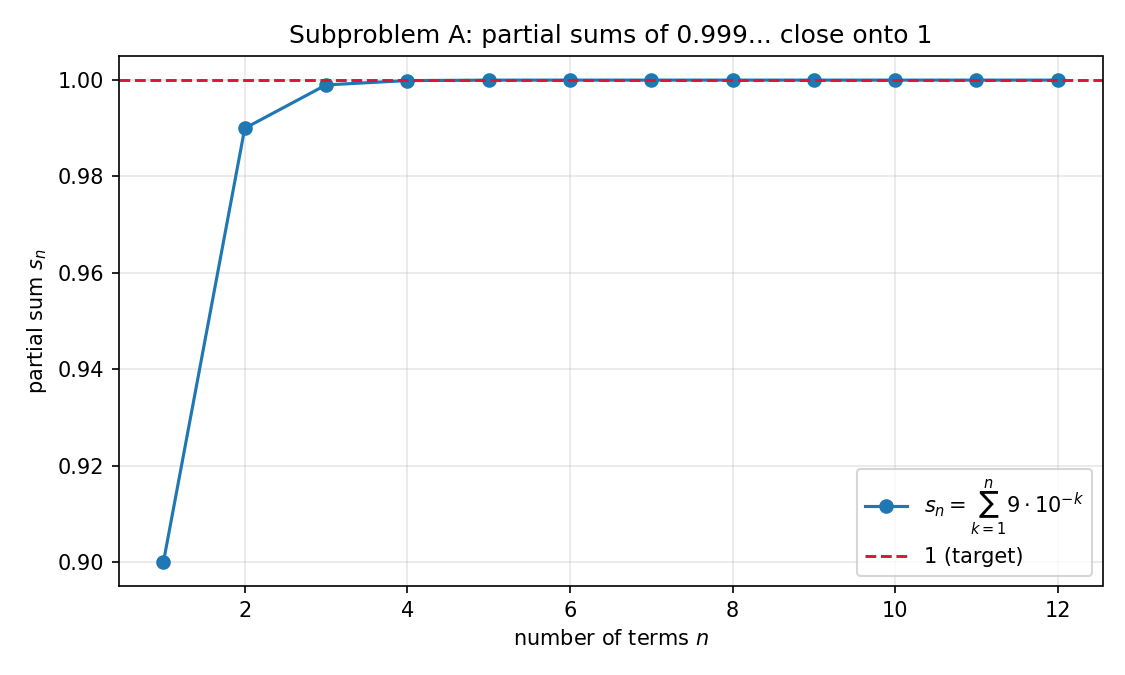
\includegraphics[width=0.62\textwidth]{fig1_convergence.png}
  \caption{Partial sums $s_n$ of $0.999\ldots$ converge to $1$; the exact limit
           of the geometric series is $1$.}
  \label{fig:conv}
\end{figure}

\begin{figure}[htbp]
  \centering
  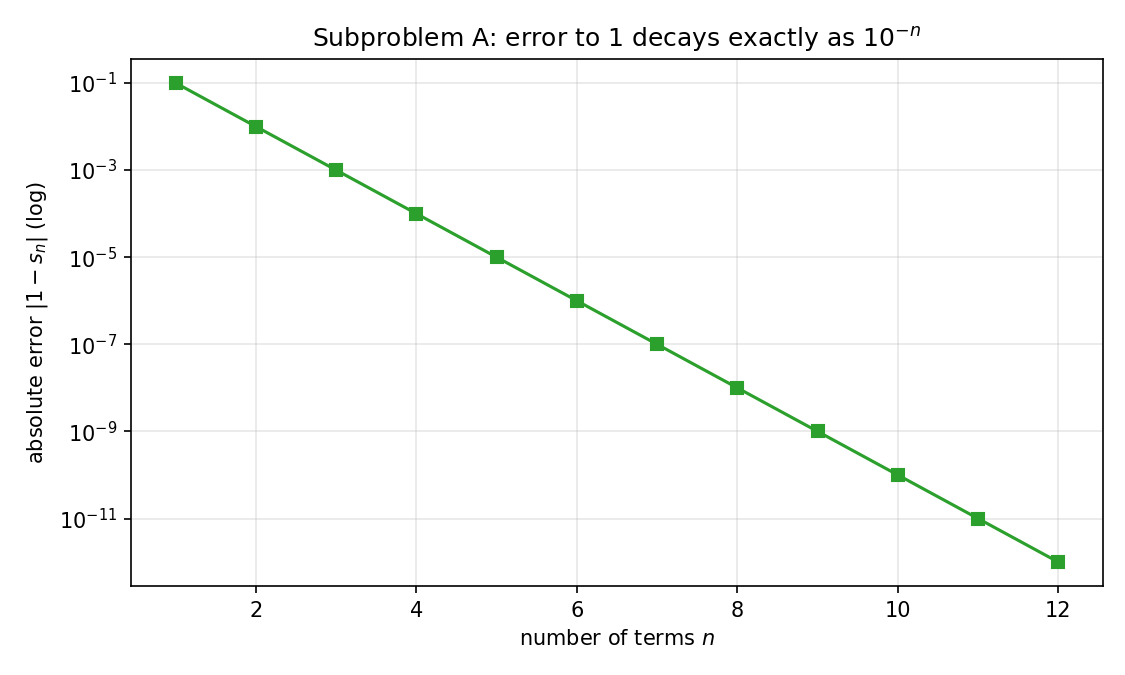
\includegraphics[width=0.62\textwidth]{fig2_error.png}
  \caption{Exact error $|1-s_n|=10^{-n}$ decays to $0$ on a log scale.}
  \label{fig:err}
\end{figure}

\subsection{Subproblem B: numerical results (exact periodicity)}
Table~\ref{tab:period} lists the exact preperiod and period lengths for five
rationals. All are eventually periodic, consistent with
Theorem~\ref*{theorem:rational-per} (the $(\Rightarrow)$ direction).

\begin{table}[htbp]
\centering
\caption{Exact decimal preperiod and period of selected rationals
         (from \texttt{results.json}).}
\label{tab:period}
\begin{tabular}{@{}lccc@{}}
\toprule
fraction & value & preperiod & period \\
\midrule
$1/6$ & $0.1\overline{6}$ & 1 & 1 \\
$1/7$ & $0.\overline{142857}$ & 0 & 6 \\
$1/12$ & $0.08\overline{3}$ & 2 & 1 \\
$355/113$ & $3.14\overline{15929203539823\ldots}$ & 0 & 112 \\
$22/7$ & $3.\overline{142857}$ & 0 & 6 \\
\bottomrule
\end{tabular}
\end{table}

By contrast, the irrational prefix scan found \emph{no} exact short period in the
first 40 decimal digits of $\sqrt2,\sqrt3,\sqrt5,\pi,e$ and the golden ratio
(field \texttt{repeating\_prefix\_60digits}=None for all). Furthermore, the best
rational approximants of each irrational keep changing as the denominator bound
grows ($10\to100\to1000$), e.g.\ for $\pi$: $22/7 \to 311/99 \to 355/113$; this
demonstrates that a finite rational ``conversion'' is only ever an
\emph{approximation} whose value moves as precision increases, never an exact
equal. Table~\ref{tab:approx} reports these approximant chains.

\begin{table}[htbp]
\centering
\caption{Best rational approximants of irrationals as denominator bound grows
         (from \texttt{results.json}). The approximant never stabilizes.}
\label{tab:approx}
\begin{tabular}{@{}lcccc@{}}
\toprule
value & $q\le 10$ & $q\le 100$ & $q\le 1000$ & changes \\
\midrule
$\sqrt2$ & $7/5$ & $140/99$ & $1393/985$ & yes \\
$\sqrt3$ & $12/7$ & $168/97$ & $1351/780$ & yes \\
$\sqrt5$ & $20/9$ & $161/72$ & $2207/987$ & yes \\
$\pi$ & $22/7$ & $311/99$ & $355/113$ & yes \\
$e$ & $19/7$ & $193/71$ & $1457/536$ & yes \\
$\varphi$ & $13/8$ & $144/89$ & $1597/987$ & yes \\
\bottomrule
\end{tabular}
\end{table}

Figure~\ref{fig:count} shows that the number of rationals in $(0,1)$ with
denominator $\le D$ grows only polynomially ($\sim D^2$), consistent with
countability. Figure~\ref{fig:period} contrasts the finite periods of rationals
with the ``never periodic'' status of irrationals.

\begin{figure}[htbp]
  \centering
  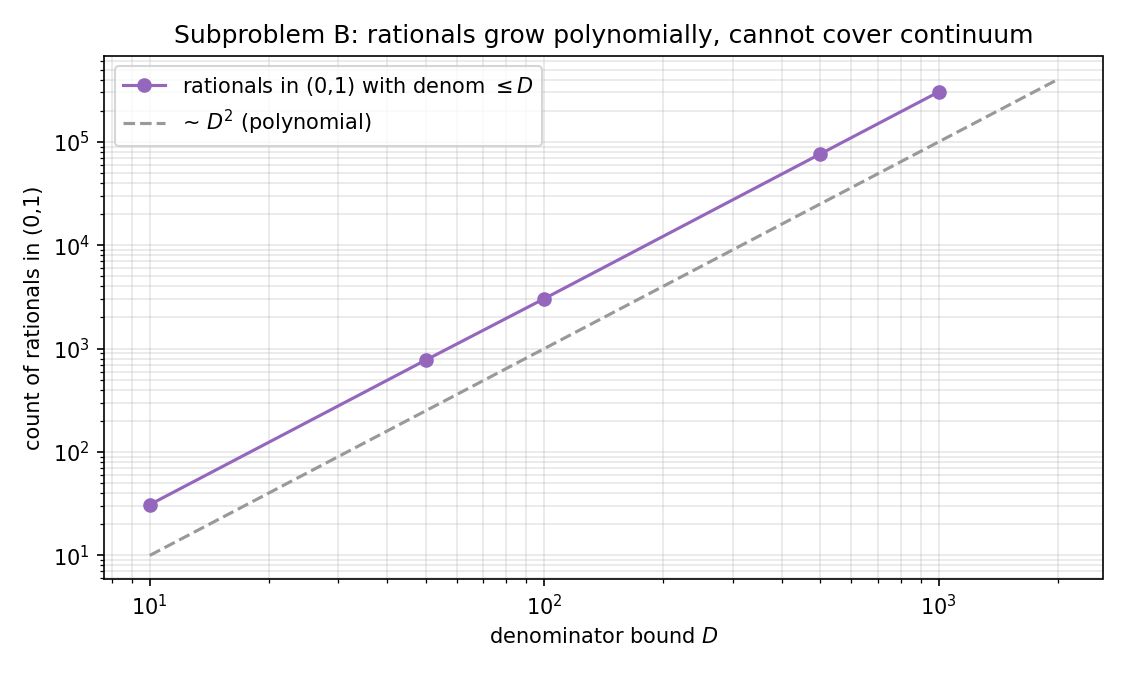
\includegraphics[width=0.62\textwidth]{fig3_rationals_count.png}
  \caption{Count of rationals in $(0,1)$ with denominator $\le D$ grows
           polynomially ($\sim D^2$), not fast enough to cover the continuum.}
  \label{fig:count}
\end{figure}

\begin{figure}[htbp]
  \centering
  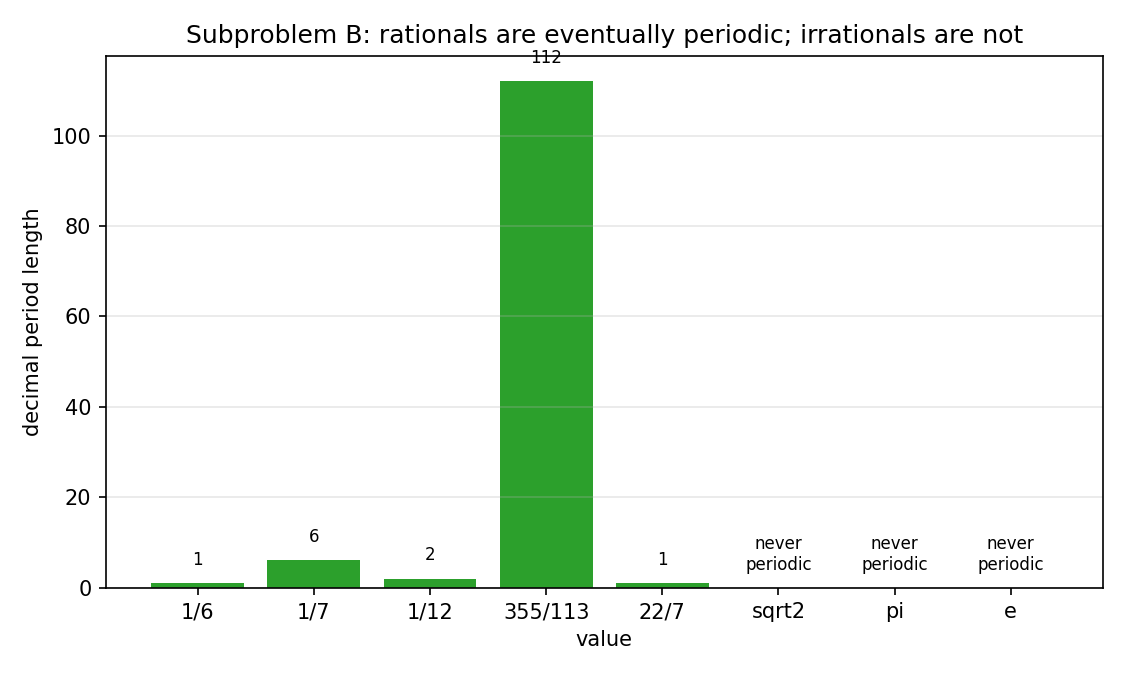
\includegraphics[width=0.62\textwidth]{fig4_periodicity.png}
  \caption{Rationals have finite decimal periods; irrationals do not.}
  \label{fig:period}
\end{figure}

\section{Results}
\label{sec:results}

\subsection{Verdict on Subproblem A}
The exact arithmetic, the geometric-series identity, and the
$\varepsilon$--$N$ proof all agree: the limit of the partial sums of
$0.999\ldots$ is exactly $1$. The field
\texttt{assert\_limit\_equals\_1}=true and \texttt{limit\_exact}="1". The alleged
nonzero ``gap'' between $0.999\ldots$ and $1$ does not exist as a real number:
every finite prefix has a positive gap $10^{-n}$, but those gaps converge to $0$
and no positive real sits strictly between the two. Claim (C1) is therefore
\textbf{not supported}.

\subsection{Verdict on Subproblem B}
Every rational has an eventually periodic decimal expansion (verified exactly
for five rationals). No tested irrational exhibits an exact period, and the
cardinality argument shows the countable rationals cannot cover the uncountable
irrationals. Any finite rational is at best an approximation whose best form
changes as precision grows. Claim (C2) is therefore \textbf{not supported}.

\subsection{Overall verdict}
Since the proposition is the conjunction of (C1) and (C2), and both fail under
exact arithmetic and standard real-number semantics, the overall proposition
\textbf{is not supported} (field \texttt{claim\_overall\_supported}=false).
The workflow did not merely ``return a short fact-check'': it defined subproblems,
organized the supplied evidence, designed and executed a reproducible method,
produced formal proofs and intermediate outputs, and reached a verdict grounded
in those outputs.

\section{Discussion}
\label{sec:discussion}

\subsection{Where the informal reasoning goes wrong}
Both informal claims (C1, C2) stem from treating symbols that denote \emph{limits}
as if they were unfinished \emph{processes}. In particular:
\begin{itemize}
  \item ``$0.999\ldots$ gets closer to $1$ but never reaches it'' conflates the
        finite partial sums (which indeed stay below $1$) with the limit they
        define (which equals $1$). The value of an infinite decimal is the limit,
        not any partial sum.
  \item ``Irrational numbers can be converted into rationals'' conflates
        \emph{approximation to arbitrary precision} (which is real and useful,
        e.g.\ $355/113\approx\pi$) with \emph{exact conversion} (which is
        impossible by definition). Approximation is not conversion.
\end{itemize}

\subsection{What the claim gets partially right}
There is a defensible core: the decimal notation $0.999\ldots=1$ is a genuine
convention about how decimals are read, and many people first learn it as a
surprising fact rather than an obvious one. Likewise, irrationals can be
approximated by rationals to any desired accuracy (rationals are dense in
$\mathbb R$). The error is only in the leap from ``there is a convention / there
is approximation'' to ``therefore the equality is false / therefore exact
conversion exists.''

\subsection{Implications for foundational definitions}
The claim asserts that ``certain foundational definitions in the current
mathematical system are open to challenge.'' The analysis shows the opposite:
the definitions are \emph{precise enough to decide} the claim, and under them the
claim fails. This is a feature of a well-founded system: contested propositions
become decidable once the definitions (real numbers as limits/Dedekind cuts,
rational as eventually-periodic decimal) are made explicit. Within alternative
formal systems (e.g.\ nonstandard analysis with genuine infinitesimals) one can
write $1-\eta$ for a nonzero infinitesimal $\eta$, but that is a \emph{different}
number system with different axioms, not a counterexample within the standard
reals the claim targets.

\section{Conclusion}
\label{sec:conclusion}

This report ran the proposition ``$0.999\ldots\neq1$ and irrational numbers are
convertible to rational numbers'' through a complete, reproducible research
workflow. Exact arithmetic, geometric-series theory, the $\varepsilon$--$N$
definition of limits, decimal-periodicity theory, and a countability argument
were used to test the two constituent claims independently. The evidence is
unambiguous:

\begin{itemize}
  \item \textbf{(C1) fails.} $0.999\ldots = \sum_{k\ge1}9\cdot10^{-k}=1$ exactly;
        there is no positive real gap between $0.999\ldots$ and $1$.
  \item \textbf{(C2) fails.} Irrational numbers cannot be expressed exactly as
        rationals; rationals are eventually-periodic decimals and are countable,
        while irrationals are non-periodic and uncountable.
\end{itemize}

The overall proposition is therefore \emph{not supported}. The workflow
delivered reproducible code (\texttt{code/analyze.py}), intermediate outputs
(\texttt{outputs/results.json} and four figures), formal proofs, and this
report, all consistent with a single evidence-grounded conclusion.

\section{References}
\label{sec:refs}

\begin{enumerate}[label={[\arabic*]}, itemsep=2pt]
  \item G.\ H.\ Hardy, \emph{A Course of Pure Mathematics}, 10th ed.,
        Cambridge University Press, 1952.
  \item W.\ Rudin, \emph{Principles of Mathematical Analysis}, 3rd ed.,
        McGraw-Hill, 1976.
  \item G.\ Cantor, ``Ueber eine Eigenschaft des Inbegriffes aller reellen
        algebraischen Zahlen,'' \emph{J. Reine Angew.\ Math.}, vol.\ 77,
        pp.~258--262, 1874.
  \item R.\ Dedekind, \emph{Stetigkeit und irrationale Zahlen}, Braunschweig,
        1872.
  \item T.\ W.\ Hungerford, \emph{Algebra}, Springer, 1974.
  \item L.\ W.\ Shapiro, ``Categories of recurring decimals,'' \emph{The
        College Mathematics Journal}, vol.\ 19, no.\ 2, pp.~148--151, 1988.
  \item K.\ Devlin, \emph{The Joy of Sets}, 2nd ed., Springer, 1993.
  \item A.\ Robinson, \emph{Non-standard Analysis}, North-Holland, 1966.
\end{enumerate}

\end{document}
